\documentclass[10pt,twocolumn,letterpaper]{article}

\usepackage{cvpr}
\usepackage{times}
\usepackage{epsfig}
\usepackage{graphicx}
\graphicspath{{./img/}}
\usepackage{amsmath}
\usepackage{amssymb}
\usepackage{textcomp}
\usepackage{hyperref}

\usepackage{listings}
\usepackage{xcolor}

\definecolor{codegreen}{rgb}{0,0.6,0}
\definecolor{codegray}{rgb}{0.5,0.5,0.5}
\definecolor{codepurple}{rgb}{0.58,0,0.82}
\definecolor{backcolour}{rgb}{0.95,0.95,0.92}

\lstdefinestyle{mystyle}{
	backgroundcolor=\color{backcolour},   
	commentstyle=\color{codegreen},
	keywordstyle=\color{orange},
	numberstyle=\tiny\color{codegray},
	stringstyle=\color{codepurple},
	%sbasicstyle=\ttfamily\footnotesize,
	basicstyle=\fontsize{5}{6}\ttfamily,
	breakatwhitespace=false,         
	breaklines=true,                 
	captionpos=b,                    
	keepspaces=true,                 
	numbers=left,                    
	numbersep=5pt,                  
	showspaces=false,                
	showstringspaces=false,
	showtabs=false,                  
	tabsize=2
}
\lstset{style=mystyle}




\usepackage[ruled,vlined]{algorithm2e}
\usepackage[italian]{babel}


\usepackage{url}

% Include other packages here, before hyperref.

% If you comment hyperref and then uncomment it, you should delete
% egpaper.aux before re-running latex.  (Or just hit 'q' on the first latex
% run, let it finish, and you should be clear).
%\usepackage[pagebackref=true,breaklinks=true,letterpaper=true,colorlinks,bookmarks=false]{hyperref}

\cvprfinalcopy % *** Uncomment this line for the final submission

\def\cvprPaperID{****} % *** Enter the CVPR Paper ID here
\def\httilde{\mbox{\tt\raisebox{-.5ex}{\symbol{126}}}}

% Pages are numbered in submission mode, and unnumbered in camera-ready
\ifcvprfinal\pagestyle{empty}\fi
\begin{document}

%%%%%%%%% TITLE
\title{PC-2019/20 Implementazione in Open-MP e CUDA dell'algoritmo K-Means}

\author{Marco Calamai\\
6314073\\
{\tt\small marco.calamai@stud.unifi.it}
% For a paper whose authors are all at the same institution,
% omit the following lines up until the closing ``}''.
% Additional authors and addresses can be added with ``\and'',
% just like the second author.
% To save space, use either the email address or home page, not both
\and
Elia Mercatanti\\
6425149\\
{\tt\small elia.mercatanti@stud.unifi.it}
}

\maketitle
\thispagestyle{empty}

%%%%%%%%% ABSTRACT
\begin{abstract}
   In questo progetto è stato implementato l'algoritmo K-Means per la clusterizzazione in tre versioni. La prima sequenziale in C++, una versione parallelizzata su CPU usando Open-MP ed un'ultima utilizzando la libreria CUDA su GPU Nvidia. Successivamente è stato fatto un confronto tra le versioni parallele e quella sequenziale per analizzare performance e speedup.
\end{abstract}

%%%%%%%%% BODY TEXT
\section{Introduction}
L'algoritmo K-Means un algoritmo di clustering, che permette di  suddividere  gruppi  di  oggetti  in  K  partizioni, chiamati cluster cluster,  sulla  base  dei  loro  attributi. Si  assume  che  gli  attributi  degli  oggetti  possano  essere  rappresentati  come  vettori. L'obiettivo  dell'algoritmo è  di  minimizzare  la  varianza  totale  intra-cluster. Ogni cluster viene identificato mediante un centroide o punto medio. L'algoritmo segue una procedura iterativa:
\begin{enumerate}
\item \textit{Inizializzazione}: seleziona K punti come centroidi iniziali scelti casualmente dall'intero datsatet.
\item \textit{Assegnameto}: assegna ogni punto del dataset al cluster più vicino in base ad una funzione di distanza dai centroidi. Come tipo distanza in questo progetto è stata utilizzata la distanza Euclidea.
\item \textit{Aggiornamento}: aggiorna i nuovi centroidi in base alla media di tutti i punti all'interno cluster
\item Ripeti i passi $2$ e $3$ fino a quando nessun punto cambia cluster.
\end{enumerate}
L'algoritmo può essere riassunto con lo pseudocodice \ref{alg:kmeans}.
\newpage

\begin{algorithm}[h]
	\SetAlgoLined  
	\DontPrintSemicolon
	\caption{K-means}
	\label{alg:kmeans}
	Seleziona K punti come centroidi iniziali.\;
	\Repeat{Gli assegnamenti non cambiano.}{
		Forma K cluster assegnando ogni punto al centroide pi\`u vicino.\;
		Ricalcola i centroidi di ogni cluster.\;
	}
\end{algorithm}


%-------------------------------------------------------------------------
\section{Implementazione sequenziale del K-Means}
Il codice dell'algoritmo K-Means sequenziale è mostrato nel codice \ref{code:sequentialK-Means}.
\subsection{Rappresentazione del Dataset, centroidi e punti}
L'implementazione sequenziale dell'algoritmo K-means è stata sviluppata in C++.\\
Punti, dataset e centroidi sono stati rappresentati come segue:
\begin{itemize}
	\item Per i punti una \textit{struct} Point con componenti:
	\begin{itemize}
		\item \textit{cluster\_id} di tipo intero per rappresentare l'etichetta del cluster a cui il punto è stato assegnato.
		\item $vector \langle int \rangle$ \textit{dimensions} per memorizzare le dimensioni del punto.
	\end{itemize}  
	
	\item Per il Dataset un $vector \langle Point \rangle$ \textit{dataset}, ovvero un vettore di \textit{struct} Point.
	\item Per ogni centroide un $vector \langle Point \rangle$ \textit{centroids}, come per il Dataset.
\end{itemize}

%-------------------------------------------------------------------------
\subsection{Inizializzazione}
I $k$ centroidi iniziali sono stati scelti in modo random da tutti i punti del dataset dato in input un valore $k$ del numero di cluster da ricercare. Una volta selezionati sono stati salvati in un vettore di Point in modo tale da essere utilizzati da tutte le varianti dell'algoritmo.\\
Questa parte è stata implementata nel file di test, comune a tutte le versioni implementate in modo tale da ri utilizzare sempre gli stessi centroidi iniziali.


\subsection{Assegnamento}
Una volta presi in input i centroidi iniziali, per ogni punto sono state misurate le distanze con ogni centroide, calcolando nel ciclo for più interno la distanza minima.\\
Il codice \ref{code:assignement} mosta nel dettaglio il metodo \textit{point\_assignement} per lo step di assegnamento. Vengono eseguiti due cicli for per iterare su ogni punto ed ogni cluster ed utilizzata una funzione \textit{calulate\_distance} per calcolare la distanza euclidea tra punto e centroide su ogni dimensione.

\begin{lstlisting}[language=c++, caption=Assegnamento sequenziale, label=code:assignement]
void points_assignment(std::vector<Point> &dataset, const int num_clusters, const std::vector<Point> &centroids) {
double min_distance, distance;
	int cluster_id;
	for (auto i = 0; i < dataset.size(); i++) {
		min_distance = std::numeric_limits<double>::max();
		for (auto j = 0; j < num_clusters; j++) {
			distance = compute_distance(dataset[i].dimensions, centroids[j].dimensions);
			if (distance < min_distance) {
				min_distance = distance;
				cluster_id = centroids[j].cluster_id;
			}
		}
		dataset[i].cluster_id = cluster_id;
	}
}
\end{lstlisting}
\subsection{Aggiornamento}
La fase di aggiornamento, eseguita nel metodo \textit{update\_centroids}, nel codice \ref{code:update}, segue tre step in tre cicli for distinti. Nel primo ciclo for vengono inizializzate a zero tutte le dimensioni di tutti i centroidi. Successivamente nel secondo step mediante un doppio ciclo for su punti e dimensioni, viene calcolata la somma di tutti i punti in ogni cluster, tenendo traccia del numero di punti in ogni partizione con un contatore. Nell'ultimo step vengono calcolate le medie vere e proprie dei punti, ovvero i centroidi aggiornati, iterando con un ciclo for sui centroidi e calcolando ognuno di essi con un semplice rapporto tra le somme precedentemente calcolate ed il contatore dei punti.
\begin{lstlisting}[language=c++, caption=Aggiornamento sequenziale, label=code:update]
void update_centroids(const std::vector<Point> &dataset, const int num_clusters, std::vector<Point> &centroids) {
	const auto num_dimensions = dataset[0].dimensions.size();
	std::vector<int> num_points_clusters(num_clusters, 0);

	// Reset the centroids.
	for (auto i = 0; i < num_clusters; i++) {
		for (auto j = 0; j < num_dimensions; j++) {
			centroids[i].dimensions[j] = 0;
		}
	}
	
	// Calculate the sums and total number of points in each cluster.
	for (auto i = 0; i < dataset.size(); i++) {
		for (auto j = 0; j < num_dimensions; j++) {
			centroids[dataset[i].cluster_id].dimensions[j] += dataset[i].dimensions[j];
		}
		num_points_clusters[dataset[i].cluster_id]++;
	}
	
	// Calculate the new centroids, for all cluster.
	for (auto i = 0; i < num_clusters; i++) {
		for (auto j = 0; j < num_dimensions; j++) {
			centroids[i].dimensions[j] /= num_points_clusters[i];
		}
	}
}
\end{lstlisting}

\subsection{Criterio d'arresto}
È stato predisposto un ciclo while dove viene controllata la convergenza dell'algoritmo, in modo tale che fino a quando gli assegnamenti dei punti ai vari cluster cambiano, vengono ripetute le fasi di assegnamento e aggiornamento. Nello specifico come mostrato nel codice \ref{code:Convergence}, il controllo viene fatto confrontando gli assegnamenti ai cluster di ogni punto tra l'iterazione corrente e quella precedente. Nel caso in cui la procedura di confronto trovi una prima differenza si continua con l'iterazione successiva.
\begin{lstlisting}[language=c++, caption=Controllo convergenza, label=code:Convergence]
bool check_convergence(const std::vector<Point> &dataset, const std::vector<Point> &old_dataset) {
	for (auto i = 0; i < dataset.size(); i++) {
		if (dataset[i].cluster_id != old_dataset[i].cluster_id) {
			return false;
		}
	}
	return true;
}
\end{lstlisting}
\begin{lstlisting}[language=c++, caption=K-Means sequenziale, label=code:sequentialK-Means]
std::tuple<std::vector<Point>, std::vector<Point>>
sequential_kmeans(std::vector<Point> dataset, const int num_clusters, std::vector<Point> centroids) {
	bool convergence = false;
	std::vector<Point> old_dataset = dataset;
	do {
		// Assignment phase, find the nearest centroid for all points, assign the point to that cluster.
		points_assignment(dataset, num_clusters, centroids);
	
		// Update phase, calculate mean of all points assigned to that cluster, for all cluster.
		update_centroids(dataset, num_clusters, centroids);
	
		// Check if the convergence criterion has been reached.
		if (check_convergence(dataset, old_dataset)) {
			convergence = true;
		} else {
			old_dataset = dataset;
		}
	} while (!convergence);
	
	return {dataset, centroids};
}
\end{lstlisting}
\section{Versioni parallele}
I due step principali dell'algoritmo (assegnamento e aggiornamento) risultano essere parallelizzabili, il primo in quanto le operazioni che vengono fatte per ogni punto sono indipendenti le une dalle altre, ed è quindi possibile prendere ogni punto, calcolare le distanze tra ogni cluster ed assegnargli quello più vicino in modo parallelo.\\
Anche il secondo step può essere eseguito in modo parallelo, facendo però attenzione durante il calcolo delle somme per l'aggiornamento dei centroidi, che devono essere fatte in modo atomico per evitare problemi di race condition.\\
Per quanto riguarda il criterio d'arresto, è stato valutato di implementarlo in modo parallelo. Le motivazioni che hanno influito nella decisione di mantenere la versione sequenziale sono due: 
\begin{enumerate}
	\item Le versioni parallele richiedono di iterare sempre e
comunque su tutto il vettore per decidere il risultato finale
del controllo mentre la versione sequenziale si può fermare non appena trova una prima differenza tra gli assegnamenti.
	\item Nella versione CUDA rendere il criterio d'arresto parallelo richiederebbe due accessi a memoria per controllo, rendendo di fatto la strategia poco performante. %A fronte della CPU che riesce a inserire in cache i vettori di assegnamento rendendo l'accesso molto più veloce. 
\end{enumerate}
Analizzando mediante il profiler di CLion l'esecuzione del codice sequenziale si è visto, come riportato in figura \ref{fig:profiler} che l'algoritmo impiega molto più tempo nel calcolo delle distanze all'interno della fase di assegnamento. Per questo motivo dovrebbero ci si potrebbe concentrare nel parallelizzare soltanto la fase di assegnamento. È stato comunque parallelizzata anche la seconda fase di aggiornamento, ottenendo in Open-MP dei piccoli miglioramenti soprattutto su dataset molto grandi.
\begin{figure}[h!]
	\centering
	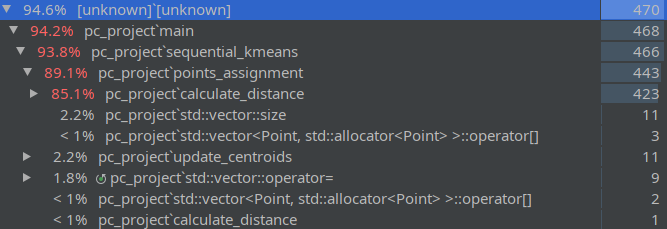
\includegraphics[scale=0.35]{Profiler.png}
	\caption{Profiler esecuzione sequenziale}
	\label{fig:profiler}
\end{figure}

\section{Implementazione parallela in Open-MP del K-Means}
Per la versione del K-Means in Open-MP, abbiamo creato all'interno del ciclo while una sezione parallela con la clausola \textit{\#pragma omp parallel} , che ingloba le due fasi del K-Means come mostrato nel codice \ref{code:pragmaparallel}. Sono state definite \textit{dataset}, \textit{num\_clusters}, \textit{centroids}, \textit{num\_points\_clusters} come variabili shared e \textit{min\_distance}, \textit{\_distance} e \textit{cluster\_id} come private.\\
Per ogni clausula è stato scelto di mantenere lo scheduler di default in quanto il carico di lavoro di tutte le iterazioni associate ai thread sono bilanciate.
\begin{lstlisting}[language=c++, caption=\#pragma omp parallel, label=code:pragmaparallel]
#pragma omp parallel num_threads(4) default(none) shared(dataset, num_clusters, centroids, num_points_clusters)
\end{lstlisting}
Per il successivo step di assegnamento è stato richiamato un \textit{\#pragma omp for} mostrato nel codice \ref{code:OMPassignement} in modo tale da parallelizzare il ciclo for più esterno del metodo e assegnare quindi un certo numero di punti ad ogni thread. La clausula \textit{\#pragma omp for} fa in modo tale che i thread non vengano ricreati ogni volta ma vengano utilizzati quelli della clausula \textit{\#pragma omp parallel} precedente evitando overhead.
\begin{lstlisting}[language=c++, caption=Assegnamento Open-MP, label=code:OMPassignement]
void
points_assignment_openmp(std::vector<Point> &dataset, const int num_clusters, const std::vector<Point> &centroids) {
	double min_distance, distance;
	int cluster_id;
	
#pragma omp for
	for (auto i = 0; i < dataset.size(); i++) {
		min_distance = std::numeric_limits<double>::max();
			for (auto j = 0; j < num_clusters; j++) {
				distance = calculate_distance_openmp1(dataset[i].dimensions, centroids[j].dimensions);
				if (distance < min_distance) {
					min_distance = distance;
					cluster_id = centroids[j].cluster_id;
				}
			}
		dataset[i].cluster_id = cluster_id;
	}
}
\end{lstlisting}
Per quanto riguarda lo step di aggiornamento, mostrato nel codice \ref{code:OMPupdate}, sono stati richiamati quattro \textit{\#pragma omp for}.\\
Il primo è stato inserito prima di un for aggiuntivo rispetto al sequenziale, utilizzato per inizializzare a zero la variabile shared \textit{num\_points\_clusters} che conta il numero di punti in ogni cluster.\\
Un secondo \textit{\#pragma omp for}, con \textit{collapse(2)} per distribuire meglio le iterazioni ad ogni thread è stato utilizzato per azzerare i centroidi.\\
Il terzo \textit{\#pragma omp for} è stato utilizzato per calcolare le somme dei punti nei cluster e contare il numero di punti in ognuno di essi. Per fare entrambe le operazioni è necessario un \textit{\#pragma omp atomic} per evitare problemi di race condition.\\
Infine, un utlimo \textit{\#pragma omp for} con \textit{collapse(2)} per fare le divisioni atomicamente come visto prima e quindi calcolare i nuovi centroidi.
\begin{lstlisting}[language=c++, caption=Aggionamento Open-MP, label=code:OMPupdate]
void update_centroids_openmp1(const std::vector<Point> &dataset, const int num_clusters, std::vector<Point> &centroids,
std::vector<int> &num_points_clusters) {
	const auto num_dimensions = dataset[0].dimensions.size();

// Reset shared num_points_clusters.
#pragma omp for
	for (auto i = 0; i < num_clusters; i++) {
		num_points_clusters[i] = 0;
	}

// Reset the centroids.
#pragma omp for collapse(2)
	for (auto i = 0; i < num_clusters; i++) {
		for (auto j = 0; j < num_dimensions; j++) {
			centroids[i].dimensions[j] = 0;
		}
	}

// Calculate the sums and total number of points in each cluster.
#pragma omp for
	for (auto i = 0; i < dataset.size(); i++) {
		for (auto j = 0; j < num_dimensions; j++) {
#pragma omp atomic
			centroids[dataset[i].cluster_id].dimensions[j] += dataset[i].dimensions[j];
		}
#pragma omp atomic
		num_points_clusters[dataset[i].cluster_id]++;
	}

// Calculate the new centroids, for all cluster.
#pragma omp for collapse(2)
	for (auto i = 0; i < num_clusters; i++) {
		for (auto j = 0; j < num_dimensions; j++) {
#pragma omp atomic
			centroids[i].dimensions[j] /= num_points_clusters[i];
		}
	}
}
\end{lstlisting}

%-------------------------------------------------------------------------
\section{Implementazione parallela in CUDA del K-Means}
\subsection{Rappresentazione del Dataset, centroidi e punti}
In CUDA Dataset e centroidi sono stati memorizzati in array bidimensionali semplici dove le colonne rappresentano le dimensioni e le righe sono i punti. Per quanto riguarda gli assegnamenti, in questo caso è stato predisposto un array unidimensionale, di lunghezza pari al numero di punti del dataset, dove ogni posizione $i$ contiene l'etichetta del cluster associato al punto $i$.\\ 
\subsection{Parallelizzazione CUDA}
Per l'implementazione dell'algoritmo K-Means in CUDA sono stati definiti $5$ kernel di cui due per lo step di assegnamento e tre per la fase di aggiornamento. Tra ognuno di essi è stato prevista una fase di sincronizzazione dei thread, in quanto l'algoritmo ha bisogno dei risultati di ogni fase precedente prima di procedere con lo step successivo.\\
Per ognuno dei kernel sono state scelte delle apposite griglie e blocchi di thread per fare in modo tale che ogni streaming multiprocessor (SM) abbia assegnato il massimo numero di threads possibile %(rispettando il massimo numero di blocchi che nel nostro caso è 32)
e allo stesso tempo che ci sia il minor numero di thread inutilizzati.%sui dataset randomici generati (nel nostro caso massimo numero di thread per SM è 2048)


\subsection{Step di assegnamento in CUDA}
Per la fase di assegnamento sono stati definiti i kernel \textit{compute\_distances} e \textit{points\_assignment}. Il primo per il calcolo delle distanze di ogni punto da ogni centroide ed il secondo per trovare, per ogni punto, il centroide più vicino ed assegnare tale punto al relativo cluster.\\
La funzione kernel \textit{compute\_distances} è mostrata nel codice \ref{code:CUDAcompdist}, dove ogni thread calcola una distanza punto - centroide. Tutte le distanze calcolate sono salvate in un array dove le righe rappresentano i punti e le colonne i centroidi. Questo array di distanze viene passato come parametro alla funzione kernel \textit{points\_assignment} mostrata nel codice \ref{code:CUDApointassign} , dove ogni thread calcola la distanza minima dai centroidi per un punto e assegna tale punto al relativo cluster.
\begin{lstlisting}[language=c++, caption=Assegnamento: \textit{compute\_distances} , label=code:CUDAcompdist]
__global__
void compute_distances(const double *device_dataset, const double *device_centroids, double *device_distances) {
	unsigned int col = blockIdx.x * blockDim.x + threadIdx.x;
	unsigned int row = blockIdx.y * blockDim.y + threadIdx.y;
	double distance = 0;
	
	if (row < const_num_points && col < const_num_clusters) {
		for (auto i = 0; i < const_num_dimensions; i++) {
			distance += pow(device_dataset[row * const_num_dimensions + i] - device_centroids[col * const_num_dimensions + i],2);
		}
		device_distances[row * const_num_clusters + col] = sqrt(distance);
	}
}

\end{lstlisting}
\begin{lstlisting}[language=c++, caption=Assegnamento: \textit{points\_assignment}, label=code:CUDApointassign]
__global__
void points_assignment(const double *device_distances, short *device_assignments) {
	int unsigned thread_id = blockDim.x * blockIdx.x + threadIdx.x;
	auto min_distance = INFINITY;
	double distance;
	short cluster_id;
	
	if (thread_id < const_num_points) {
		for (auto i = 0; i < const_num_clusters; i++) {
			distance = device_distances[thread_id * const_num_clusters + i];
			if (distance < min_distance) {
				min_distance = distance;
				cluster_id = i;
			}
		}
	device_assignments[thread_id] = cluster_id;
	}
}
\end{lstlisting}
\subsection{Step di aggiornamento in CUDA}
Per la fase di aggiornamento sono stati definiti i kernel \textit{initialize\_centroids}, \textit{compute\_sums} e \textit{update\_centroids}. Il primo si occupa di inizializzare a zero il valore dei centroidi dove ogni thread pone a zero una coppia centroide - dimensione, come mostrato nel codice \ref{code:CUDAinizcentr}.\\
La funzione kernel \textit{compute\_sums}, mostrata nel codice \ref{code:CUDAcomputesums}, si occupa, per ogni cluster, di sommare tutti i punti in esso e calcolare il loro numero. Nello specifico ogni thread gestisce una coppia punto - dimensione eseguendo le operazioni in modo atomico per evitare race condition. In questo modo l'incremento del contatore avviene per ogni dimensione del punto, quindi al momento dell'aggiornamento dei centroidi andrà diviso per il numero di dimensioni.\\
La funzione kernel \textit{update\_centroids}, mostrata nel codice \ref{code:CUDAupdatecentroids}, si occupa di calcolare i centroidi aggiornati dove ogni thread gestisce una coppia cluster - dimensione.\\
\begin{lstlisting}[language=c++, caption=Aggiornamento: \textit{initialize\_centroids}, label=code:CUDAinizcentr]
__global__
void initialize_centroids(double *device_centroids) {
	int unsigned col = blockDim.x * blockIdx.x + threadIdx.x;
	int unsigned row = blockDim.y * blockIdx.y + threadIdx.y;
	
	if (row < const_num_clusters && col < const_num_dimensions) {
		device_centroids[row * const_num_dimensions + col] = 0;
	}
}
\end{lstlisting}
\begin{lstlisting}[language=c++, caption=Aggiornamento: \textit{compute\_sums}, label=code:CUDAcomputesums]
__global__
void compute_sums(double *device_centroids, const double *device_dataset, const short *device_assignments,
	int *device_count) {
	int unsigned col = blockDim.x * blockIdx.x + threadIdx.x;
	int unsigned row = blockDim.y * blockIdx.y + threadIdx.y;
	
	if (row < const_num_points && col < const_num_dimensions) {
		short cluster_id = device_assignments[row];
		doubleAtomicAdd(&(device_centroids[cluster_id * const_num_dimensions + col]),
		device_dataset[row * const_num_dimensions + col]);
		atomicAdd(&(device_count[cluster_id]), 1);
	}
}
\end{lstlisting}
\begin{lstlisting}[language=c++, caption=Aggiornamento: \textit{update\_centroids}, label=code:CUDAupdatecentroids]
__global__
void update_centroids(double *device_centroids, const int *device_count) {
	int unsigned col = blockDim.x * blockIdx.x + threadIdx.x;
	int unsigned row = blockDim.y * blockIdx.y + threadIdx.y;
	
	if (row < const_num_clusters && col < const_num_dimensions) {
		device_centroids[row * const_num_dimensions + col] =
		device_centroids[row * const_num_dimensions + col] / (double(device_count[row]) / const_num_dimensions);
	}
}
\end{lstlisting}





%-------------------------------------------------------------------------
\section{Test e risultati}
I test sono stati eseguiti su CPU quad core i7 3770K e GPU Nvidia GTX 1080.\\
I centroidi iniziali sono stati selezionati in modo random da tutto il dataset e riutilizzati per l'esecuzione di ogni versione del K-Means.\\
Per ogni versione è stato calcolato il tempo di esecuzione e lo speed-up ottenuto rispetto alla versione sequenziale.\\
I test sono stati eseguiti sia su datasets random che su datasets reali.\\
I dataset random sono stati generati variando numero di punti e numero di dimensioni e l'algoritmo K-Means è stato eseguito al variare del numero di cluster da ricercare tra $10$, $100$ e $1000$.\\
Nella tabella in figura \ref{fig:tablerandomdatasets} sono mostrati i risultati ottenuti con le tre versioni del K-Means implementate su datasets random.\\
Dai risultati ottenuti si può vedere come al crescere della dimensione del problema, la versione Open-MP raggiunge uno speed-up quasi lineare, pari circa a 4, sulla CPU di test. Dalla tabella si nota che lo speed-up di entrambe le versioni parallele incrementa % all'aumentare del numero di punti ma soprattutto 
all'aumentare del numero di clusters e dimensioni in quanto si aumenta il carico di lavoro, soprattutto per la parte relativa al calcolo delle distanze.\\
Entrambe le versioni parallele risultano decisamente più efficienti della versione sequenziale, soprattutto quella in CUDA dove si ottengono tempi di esecuzione notevolmente più bassi.\\
Per quanto riguarda i risultati ottenuti su datasets reali mostrati in figura \ref{fig:tablerealdatasets} e descritti in \ref{fig:tabledescriptiondatasets} le considerazioni fatte precedentemente sono confermate.\\
\begin{figure}[h!]
	\centering
	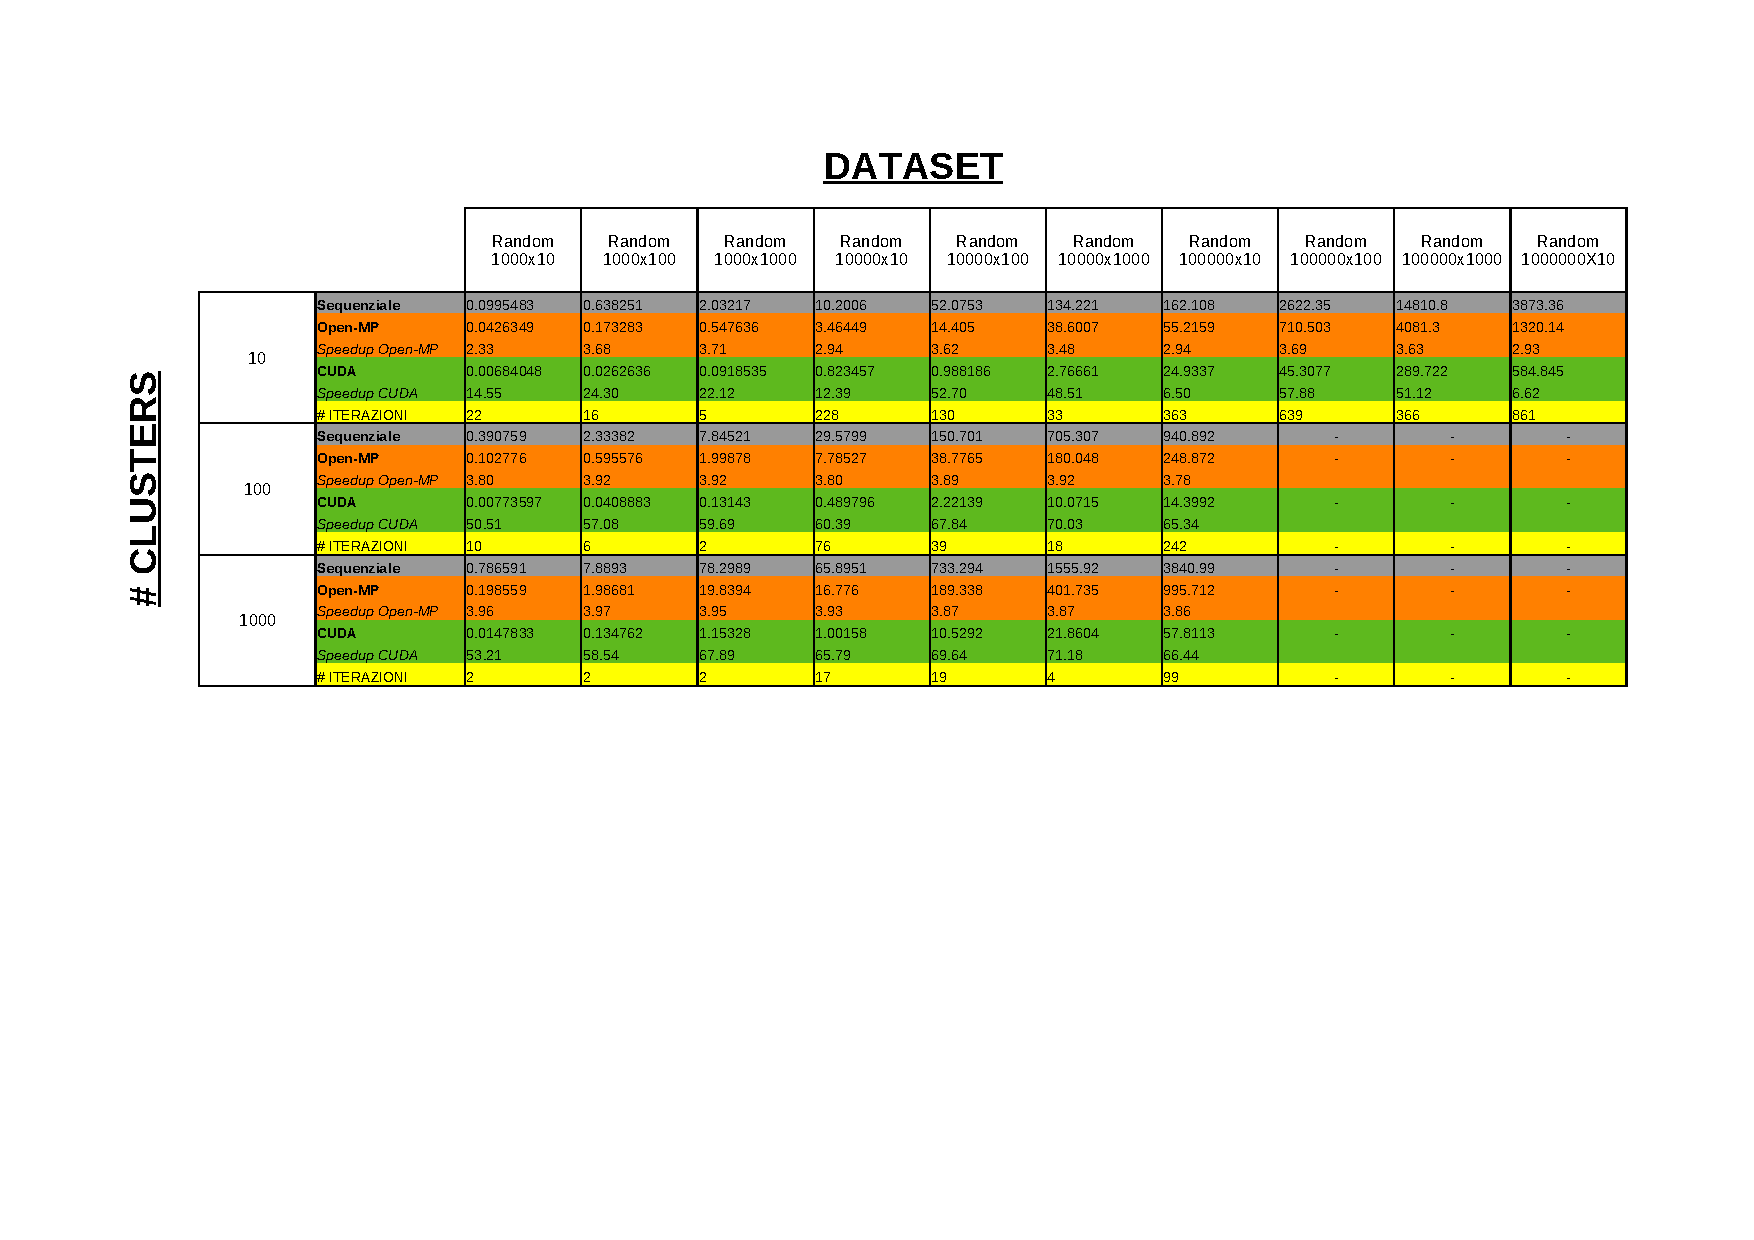
\includegraphics[scale=0.7]{TableResults.pdf}
	\caption{Results on random datasets}
	\label{fig:tablerandomdatasets}
\end{figure}
\begin{figure}[h!]
	\centering
	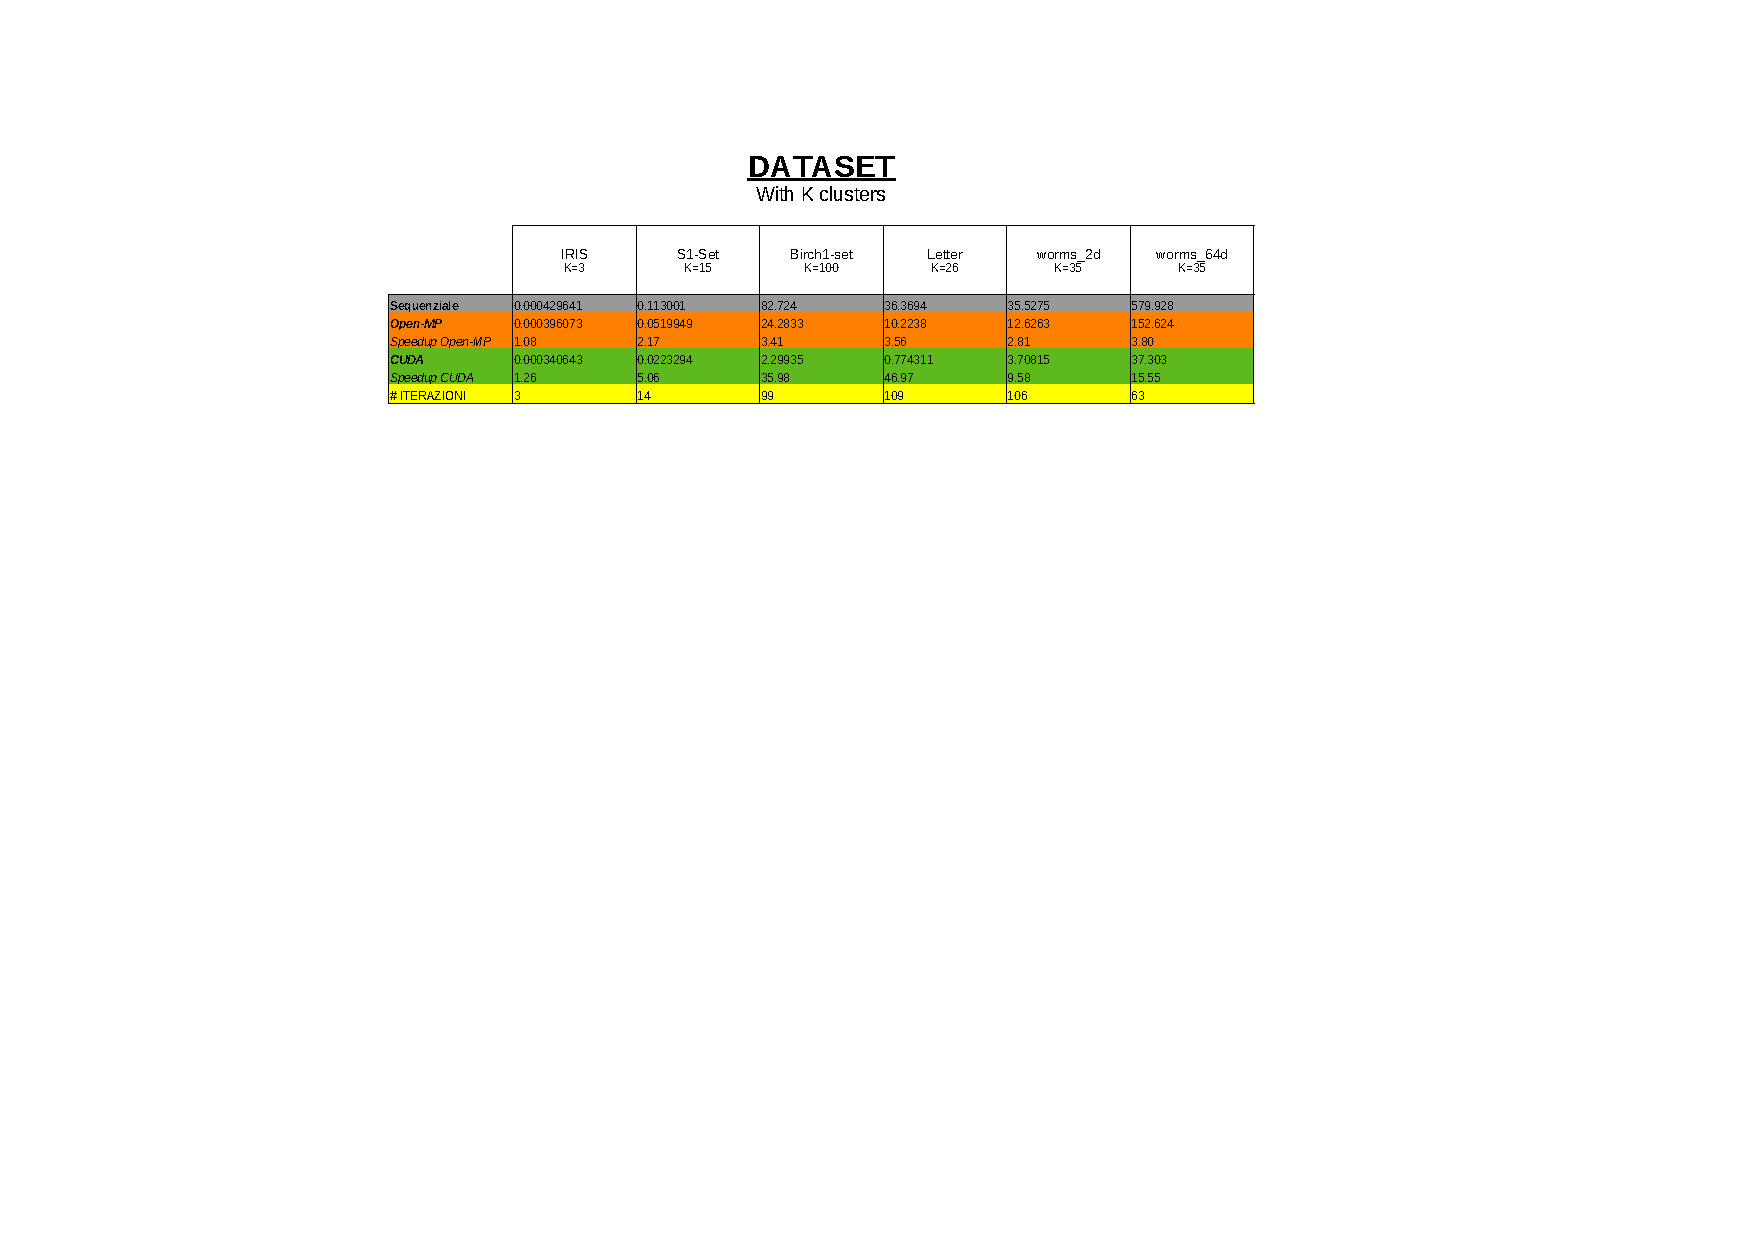
\includegraphics[scale=0.9]{TableResults2.pdf}
	\caption{Results on real datasets}
	\label{fig:tablerealdatasets}
\end{figure}

\begin{figure}[h!]
	\centering
	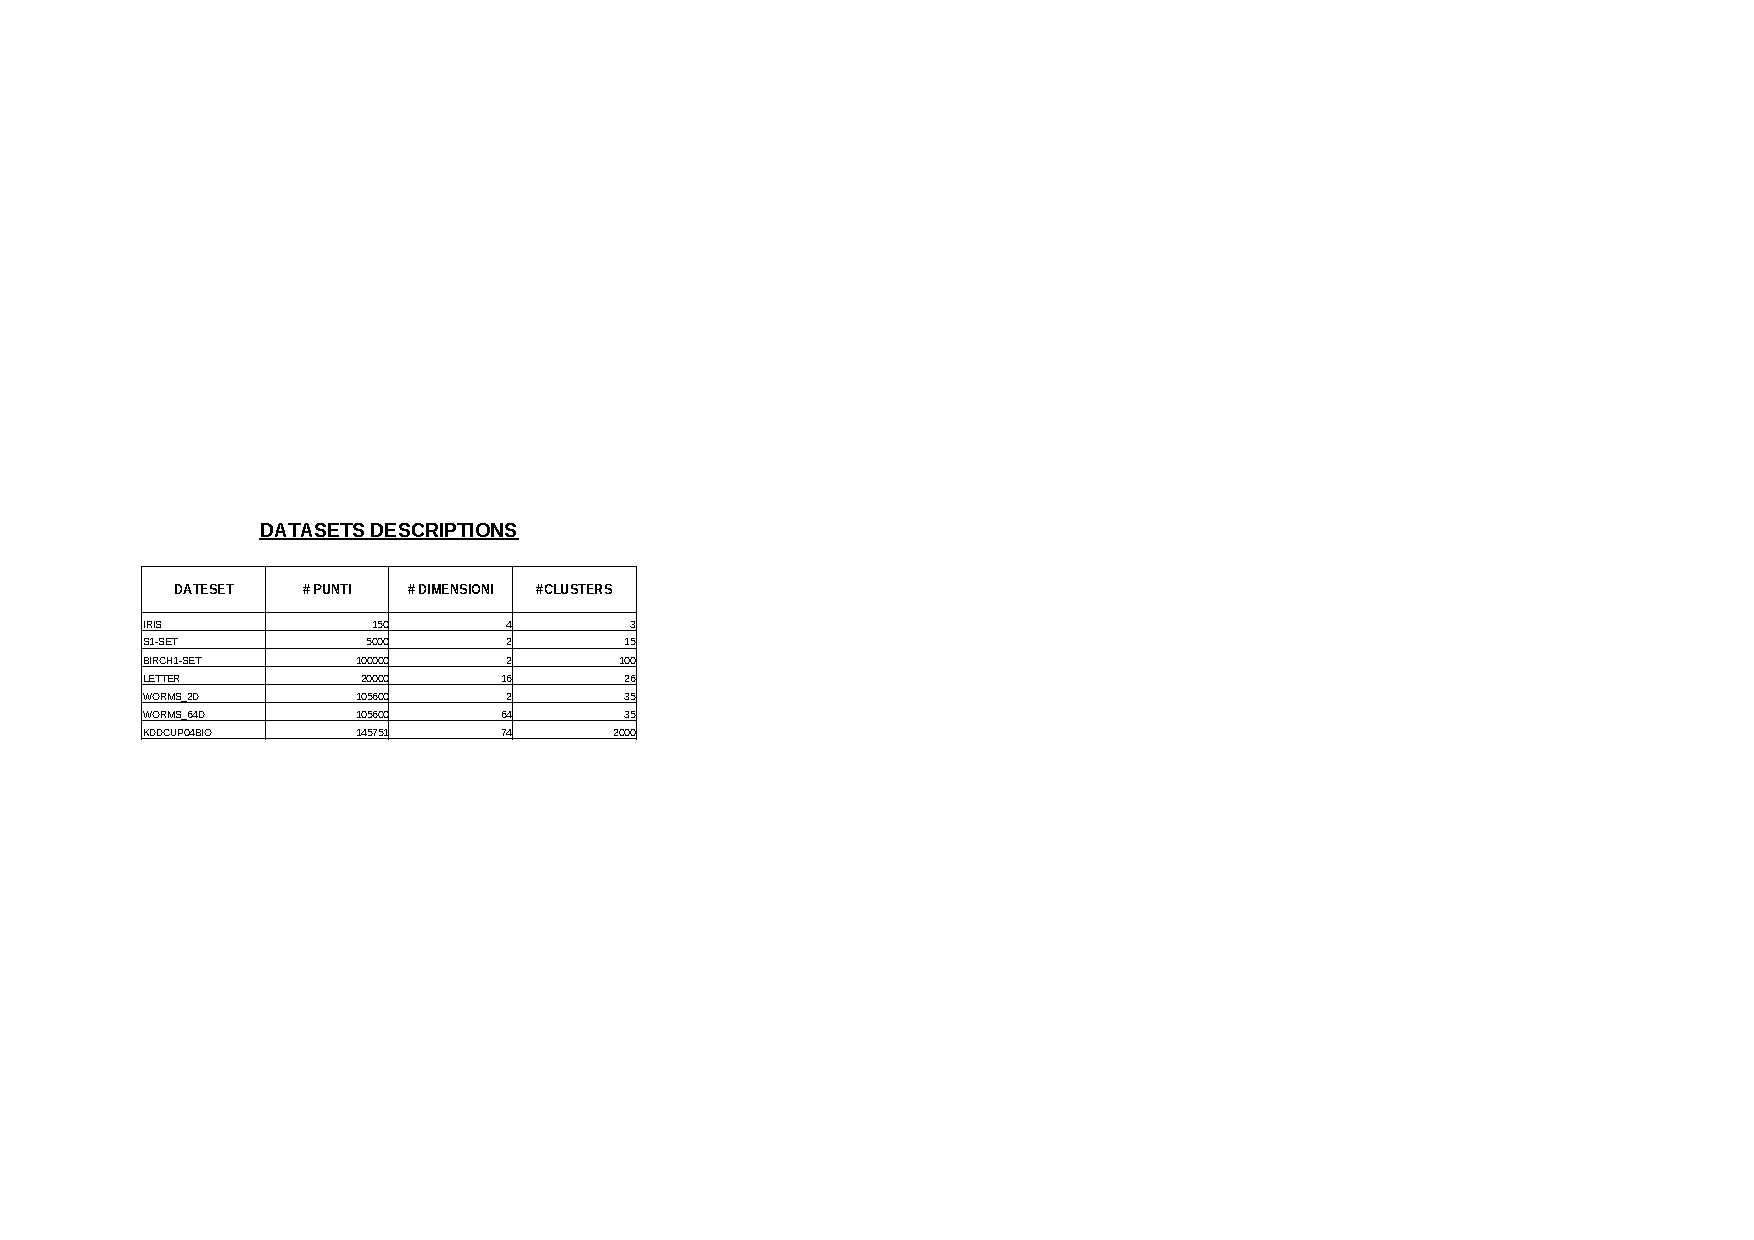
\includegraphics[scale=0.7]{TableDatasetDescription.pdf}
	\caption{Datasets descripions}
	\label{fig:tabledescriptiondatasets}
\end{figure}


%-------------------------------------------------------------------------


\section{GitHub}

\href{https://github.com/elia-mercatanti/pc-project}{https://github.com/elia-mercatanti/pc-project}\\
Per eseguire le tre versioni del K-Means (sequenziale, Open-MP e CUDA) su datasets locali è necessario passare al programma il percorso del dataset e il numero di cluster da ricercare. Il file test.cpp si occuperà di testare il dataset selezionato con tutte le versioni dell'algoritmo.\\
Nel caso in cui non venga passato nessun parametro al programma allora il file test.cpp si occuperà di generare tutti i datsets random visti precedentemente (nel caso in cui non siano già stati creati) e terminerà l'esecuzione.


\end{document}
